\documentclass{article}
\usepackage{tkz-tab}
\usepackage{amsmath} 
\usepackage{geometry}
\usepackage{indentfirst}
\setlength{\parindent}{0cm} % Retrait du paragraphe
\geometry{
    left=1cm }
\begin{document}
\underline{Tableau de variation de $f(x)$}\\
                   
$f(x)=\frac{\left(x - 2\right) \left(x - 1\right)}{x}$\\
$f'(x)=\frac{x - 2}{x} + \frac{x - 1}{x} - \frac{\left(x - 2\right) \left(x - 1\right)}{x^{2}}$\\

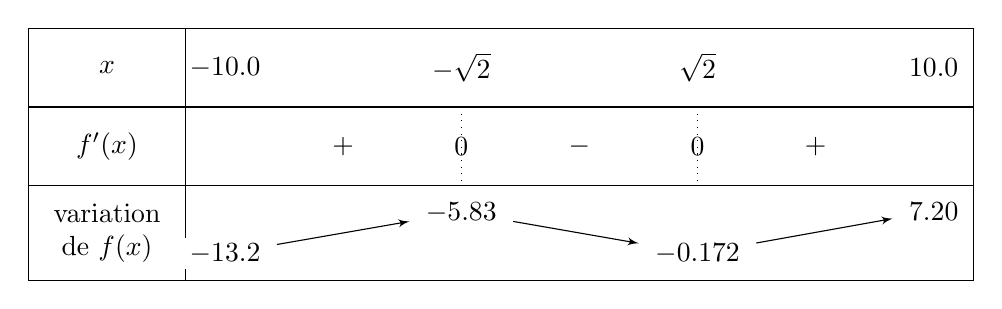
\begin{tikzpicture}
\tkzTabInit[espcl=3]{$x$ / 1 , $f'(x)$ / 1, variation de $f(x)$/1.2}
{$-10.0$,$- \sqrt{2}$,$\sqrt{2}$,$10.0$}
\tkzTabLine{,+,z,-,z,+}
\tkzTabVar{-/$-13.2$,+/$-5.83$,-/$-0.172$,+/$7.20$}
\end{tikzpicture}
\end{document}